% В этом документе преамбула

%%% Работа с русским языком
\usepackage{cmap}					% поиск в PDF
\usepackage{mathtext} 				% русские буквы в формулах
\usepackage[T2A]{fontenc}			% кодировка
\usepackage[utf8]{inputenc}			% кодировка исходного текста
\usepackage[english,russian]{babel}	% локализация и переносы
\usepackage{indentfirst}			% чтобы первый абзац в разделе отбивался красной строкой
\frenchspacing						% тонкая настройка пробелов

%%% Приведение начертания букв и знаков к русской типографской традиции
\renewcommand{\epsilon}{\ensuremath{\varepsilon}}
\renewcommand{\phi}{\ensuremath{\varphi}}			% буквы "эпсилон"
\renewcommand{\kappa}{\ensuremath{\varkappa}}		% буквы "каппа"
\renewcommand{\le}{\ensuremath{\leqslant}}			% знак меньше или равно
\renewcommand{\leq}{\ensuremath{\leqslant}}			% знак меньше или равно
\renewcommand{\ge}{\ensuremath{\geqslant}}			% знак больше или равно
\renewcommand{\geq}{\ensuremath{\geqslant}}			% знак больше или равно
\renewcommand{\emptyset}{\varnothing}				% знак пустого множества

%%% Дополнительная работа с математикой
\usepackage{amsmath,amsfonts,amssymb,amsthm,mathtools} % AMS
\usepackage{icomma} % "Умная" запятая: $0,2$ --- число, $0, 2$ --- перечисление

%% Номера формул
\mathtoolsset{showonlyrefs=true} % Показывать номера только у тех формул, на которые есть \eqref{} в тексте.

%% Свои команды

% операции, не определённые (или имеющие иные обохначения) в мат. пакетах
\DeclareMathOperator{\sgn}{\mathop{sgn}}				% ф-ия sgn
\renewcommand{\tg}{\mathop{\mathrm{tg}}\nolimits}		% обозначение тангенса

%% Перенос знаков в формулах (по Львовскому)
\newcommand*{\hm}[1]{#1\nobreak\discretionary{}
{\hbox{$\mathsurround=0pt #1$}}{}}

%%% Работа с картинками
\usepackage{graphicx}  % Для вставки рисунков
\graphicspath{{images/}{images2/}}  % папки с картинками
\setlength\fboxsep{3pt} % Отступ рамки \fbox{} от рисунка
\setlength\fboxrule{1pt} % Толщина линий рамки \fbox{}
\usepackage{wrapfig} % Обтекание рисунков текстом

%%% Работа с таблицами
\usepackage{array,tabularx,tabulary,booktabs} % Дополнительная работа с таблицами
\usepackage{longtable}  % Длинные таблицы
\usepackage{multirow} % Слияние строк в таблице

%%% Теоремы
\theoremstyle{plain} % Это стиль по умолчанию, его можно не переопределять.
\newtheorem{theorem}{Теорема}[section]
\newtheorem{lemma}{Лемма}[section]
\newtheorem{definition}[theorem]{Определение}
\newtheorem{property}{Свойство}
 
\theoremstyle{definition} % "Определение"
\newtheorem{corollary}{Следствие}[theorem]
\newtheorem{exmp}{Пример}[section]
 
\theoremstyle{remark} % "Примечание"
\newtheorem*{nonum}{Решение}
\newtheorem*{evidence}{Доказательство}
\newtheorem*{remark}{Примечание}

%%% Программирование
\usepackage{etoolbox} % логические операторы

%%% Страница
\usepackage{extsizes} % Возможность сделать 14-й шрифт
\usepackage{geometry} % Простой способ задавать поля
	\geometry{top=25mm}
	\geometry{bottom=35mm}
	\geometry{left=35mm}
	\geometry{right=20mm}

%\usepackage{fancyhdr} % Колонтитулы
% 	\pagestyle{fancy}
 	%\renewcommand{\headrulewidth}{0pt}  % Толщина линейки, отчеркивающей верхний колонтитул
% 	\lfoot{Нижний левый}
% 	\rfoot{Нижний правый}
% 	\rhead{Верхний правый}
% 	\chead{Верхний в центре}
% 	\lhead{Верхний левый}
%	\cfoot{Нижний в центре} % По умолчанию здесь номер страницы

\usepackage{setspace} % Интерлиньяж (межстрочные интервалы)
%\onehalfspacing % Интерлиньяж 1.5
%\doublespacing % Интерлиньяж 2
%\singlespacing % Интерлиньяж 1

\usepackage{lastpage} % Узнать, сколько всего страниц в документе.

\usepackage{soulutf8} % Модификаторы начертания

\usepackage{hyperref}
\usepackage[usenames,dvipsnames,svgnames,table,rgb]{xcolor}
\hypersetup{				% Гиперссылки
    unicode=true,           % русские буквы в раздела PDF
    pdftitle={Заголовок},   % Заголовок
    pdfauthor={Автор},      % Автор
    pdfsubject={Тема},      % Тема
    pdfcreator={Создатель}, % Создатель
    pdfproducer={Производитель}, % Производитель
    pdfkeywords={keyword1} {key2} {key3}, % Ключевые слова
    colorlinks=true,       	% false: ссылки в рамках; true: цветные ссылки
    linkcolor=MidnightBlue,          % внутренние ссылки
    citecolor=black,        % на библиографию
    filecolor=magenta,      % на файлы
    urlcolor=blue           % на URL
}

\usepackage{csquotes} % Еще инструменты для ссылок

%\usepackage[style=authoryear,maxcitenames=2,backend=biber,sorting=nty]{biblatex}

\usepackage{multicol} % Несколько колонок

%%% Работа с графикой
\usepackage{tikz}
\usetikzlibrary{calc}
\usepackage{tkz-euclide}
\usetikzlibrary{arrows}
\usepackage{pgfplots}
\usepackage{pgfplotstable}

%%% Настройка подписей к плавающим объектам
\usepackage{floatrow}	% размещение
\usepackage{caption}	% начертание
\captionsetup[figure]{labelfont=bf,textfont=it,font=footnotesize}	% нумерация и надпись курсивом
% для подфигур: заголовок подписи полужирный, текст заголовка обычный
% выравнивание является неровным (т.е. выровненным по левому краю)
% singlelinecheck = off означает, что настройка выравнивания используется, даже если заголовок имеет длину только одну строку.
% если singlelinecheck = on, то заголовок всегда центрируется, когда заголовок состоит только из одной строки.
\captionsetup[subfigure]{labelfont=bf,textfont=normalfont,singlelinecheck=off,justification=raggedright}

%%% Stuff для графиков и рисунков



\title{Теория вероятностей и мат. статистика \\ ИДЗ1}
\date{28.03.2020}
\author{Почаев Никита Алексеевич, гр. 8381 \\ \href{mailto:pochaev.nik@gmail.com}{pochaev.nik@gmail.com} \\ Преподаватель: Малов Сергей Васильевич}

\begin{document}
	
\renewcommand{\figurename}{Рисунок}

\maketitle

\begin{figure}[H]
	\center{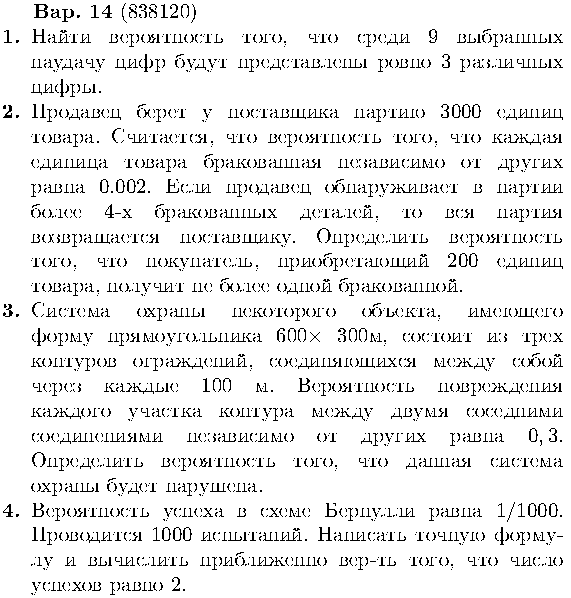
\includegraphics[scale=1]{./media/Задание.pdf}}
\end{figure}

\section*{Задача 1.}

Для удобства обозначений будем называть выбранные цифры \textit{разрядами}, т.е. 9 выбранных цифр образуют 9-ти разрядную комбинацию (не число, т.к. мы в том числе учитываем варианты, где в начале могут стоять 0-ли). Кол-во таких комбинаций будет определяться по ф-ле числа размещений с повторениями: $\# \Omega = A_n^{-k} = A_{10}^{-9} = 10^9 = 1000000000$.

Событие $A$ - 9-ти значная комбинация содержит ровно 3 различные цифры.

Способов выбрать 3 разные цифры из всех доступных ($0-9$): $C_{10}^3 = \dfrac{10!}{3! \cdot (10-3)!} = 120$. 

Из 3-х цифр можно составить $A_n^{-k} = 3^9$ 9-ти разрядных комбинаций. Из них необходимо вычесть комбинации, составленные только из 2-х или 1-ой цифр (пользуемся формулой включения исключения), т.е. $C_3^2 \cdot (2^9 - 2)$ (3 позиции на которой может стоять одна из 2-х взятых из 9-ти выбранных цифр, минус 2 варианта включённых дважды), тут же замечаем, что вычли комбинации по типу $111111111111$ по два раза $\Rightarrow$ прибавляем их. В итоге: $3^9 - C_3^2 \cdot (2^9 - 2) + 3 = 18156$.

\[ \Rightarrow P(A) = \frac{\# A}{\# \Omega} = \frac{C_{10}^3 \cdot (3^9 - C_3^2 \cdot (2^9 - 2) - 3)}{10^9} = \frac{120 \cdot 18156}{1000000000} = 0.00217872 \]

\noindent \textbf{Ответ:} 0.00217872

\section*{Задача 2.}

\begin{center}
	\fbox{%
		\parbox[t][4cm]{13cm}{%
			Если количество испытаний $n$ достаточно велико, а вероятность $p$ появления события $A$ в отдельно взятом испытании весьма мала (0,05-0,1 и меньше), то вероятность того, что в данной серии испытаний событие $A$ появится ровно $m$ раз, можно приближенно вычислить по формуле Пуассона:
			\[ P_m \approx \frac{\lambda^m}{m!} \cdot e^{- \lambda} \]
			где $\lambda = np$.
	}}\qquad
\end{center}

Покупатель сможет приобрести товар у продавца только в том случае, если в партии из 3000 единиц товара будет от 0 до 4 бракованных детали. Событие $B_i$ - партии оказалось $i \in [0-4]$ бракованных деталей. Количество испытаний - единиц товаров в партии велика, а вер-ть неисправности одной мала $\Rightarrow$ можно использовать ф-лу Пуассона и получить вероятность того, что в партии будет следующее количество бракованных деталей:
\[ \lambda = np = 3000 \cdot 0.002 = 6 \]
\[ P(B_0) = \frac{6^0}{0!} \cdot e^{-6} \approx 0.002478752 ~~~~~~~~~ P(B_1) = \frac{6^1}{1!} \cdot e^{-6} \approx 0.014872513 \]
\[ P(B_2) = \frac{6^2}{2!} \cdot e^{-6} \approx 0.044617539 ~~~~~~~~~ P(B_3) = \frac{6^3}{3!} \cdot e^{-6} \approx 0.089235078 \]
\[ P(B_4) = \frac{6^4}{4!} \cdot e^{-6} \approx 0.133852618 \]
Событие $A$ - партия будет выставлена на продажу продавцом:
\[ P(A) = \sum_{i=0}^{4} P(B_i) = 0.002478752 + 0.014872513 + 0.044617539 + 0.089235078 + 0.133852618 = 0.2850565 \]

Считаем, что продавец перебирает всю партию и если находит $\le 4$ бракованных деталей, то отправляет её всю (в том числе бракованные детали) в продажу. Таким образом, мы гарантировано знаем, что в поступивших в продажу 3000 деталях будет $\le 4$ бракованных.

Пересчитаем найденные вероятности в условные: в партии $i \in [0-4]$ бракованных деталей, при условии, что она поступила в продажу - событие $A$. Если событие $A$ выполнено, то в партии точно меньше 4 бракованных.
\[ P(B_i|A) = \frac{P(B_i \cap A)}{P(A)} \]
\[ P(B_i \cap A) = P(B_i) P(A|B_i) = P(B_i) , \]
т.к. $P(A|B_i) = 1$ - если в партии $\le 4$ бракованных деталей, она обязательно поступает в продажу
\[ \Rightarrow P(B_i|A) = \frac{P(B_i)}{P(A)} \]

Таким образом,
\begin{table}[H]
	\centering
	\begin{tabular}{|c|c|c|c|c|c|}
		\hline
		$i$        & 0           & 1           & 2           & 3           & 4           \\ \hline
		$P(B_i|A)$ & 0.008695667 & 0.052173913 & 0.156521739 & 0.313043477 & 0.469565220 \\ \hline
	\end{tabular}
\end{table}
\[ \sum_{i=0}^{4} P(B_i|A) = 1 \Rightarrow \text{это ПГС} \]

Событие $C$ - среди 200 единиц товара из 3000-ой партии будет \textit{не более одной} бракованной.
\begin{table}[H]
	\centering\makegapedcells
	\begin{tabular}{|c|c|c|c|c|c|}
		\hline
		$i$        & 0           & 1           & 2                                         & 3                                                                                          & 4                                                                                                                                   \\ \hline
		$P(C_i)$   & 1           & 1           & $1 - \frac{C_{3000}^{2}}{C_{3000}^{200}}$ & $1 - \left(\frac{C_{3000}^{2}}{C_{3000}^{200}}+\frac{C_{3000}^{3}}{C_{3000}^{200}}\right)$ & $1 - \left(\frac{C_{3000}^{2}}{C_{3000}^{200}} + \frac{C_{3000}^{3}}{C_{3000}^{200}} + \frac{C_{3000}^{4}}{C_{3000}^{200}} \right)$ \\ \hline
		$P(B_i|A)$ & 0.008695667 & 0.052173913 & 0.156521739                               & 0.313043477                                                                                & 0.469565220                                                                                                                         \\ \hline
	\end{tabular}
\end{table}

По формуле полной группы событий: $P(C) = \sum\limits_{i=0}^{4} P(B_i|A)P(C_i)$

Отметим, что даже при наличии 4-х бракованных деталей в партии, вероятность, что покупатель получит хотя бы одну слишком мала. Соответствующие вычисления приведены в прикреплённом блокноте Wolfram Mathematica. Таким образом, можно утверждать, что итоговая вероятность того, что покупатель получит $\le 1$ бракованной детали будет стремится к единицу (т.к. события $P(B_i|A)$ образуются ПГС).

\noindent \textbf{Ответ:} $\approx 1$

\section*{Задача 3.}

\begin{figure}[H]
	\center{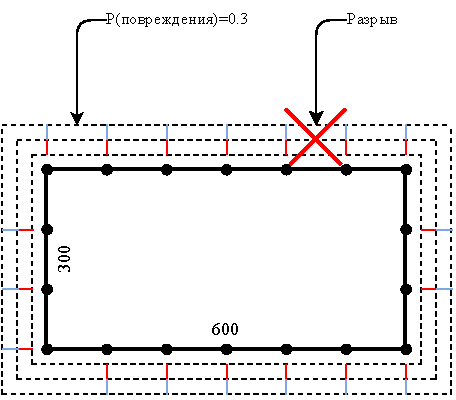
\includegraphics[scale=1.3]{./media/Периметр.pdf}}
\end{figure}

Событие $A$ - охранная система была нарушена.

По условию задачи условием нарушения безопасности является разрыв соединения у всех трёх контуров в едином месте. Рассмотрим один такой фрагмент, вероятность его разрыва: $0.3^3 = 0.027$. Охранная система будет нарушена, если произошёл хотя бы один разрыв (возможно и больше), таким образом, вероятность данного событие ($B$) равна: 1 - вероятность, что абсолютно все участки не были разрушены. Вероятность, что целостность какого-то участка не нарушилась: $1-0.3^3$. Всего таких участков 18 $\Rightarrow$
\[ P(B) = (1 - 0.3^3)^{18} = 0.610985811 \]
В результате:
\[ P(A) = 1 - P(B) = 1 - 0.610985811 = 0.389014189 \]

\noindent \textbf{Ответ:} 0.389014189

\section*{Задача 4.}

Точная формула:
\[ P(\mu_{1000} = 2) = C_{1000}^{2} \left(\frac{1}{1000}\right)^{2} \left( 1 - \frac{1}{1000} \right)^{1000-2} = 499500 \cdot 10^{-6} \cdot 0.368431920 \approx 0.184031744 \]

Заметим, что выполнено условие для для применения формулы Пуассона:
\[ \lambda = np = \frac{1}{1000} \cdot 1000 = 1 \le 10 \]
Таким образом, приближённая вероятность равна:
\[ P(\mu_{1000}=2) \approx \frac{\lambda^{2}}{2} \cdot e^{-\lambda} \approx 0.183940 \]

\textbf{Дополнительно:}

В данном случае не выполнено условие для применения теоремы Муавра-Лапласа ($\lambda \not > 10$), однако, попробуем воспользоваться ею, что оценки точности.

Из локальной предельной теоремы Муавра-Лапласа следует приближенная формула:
\[ P_n(m) \approx \frac{1}{\sqrt{npq}} \cdot \phi \left( \frac{m - np}{\sqrt{npq}} \right) \]
где $\phi(x) = \frac{1}{\sqrt{2 \pi}} e^{-\frac{x_k^2}{2}}$.

Приближённая вероятность таким образом будет равна:
\[ P(\mu_{1000} = 2) \approx \frac{1}{\sqrt{np(1-p)}\sqrt{2 \pi}} \cdot e^{-\frac{x_k^2}{2}} \approx \]
Учитывая, что:
\[ p = 0.001, q = 0.999 \]
\[ x_k^2 = \left( \frac{k-np}{\sqrt{np(1-p)}} \right)^2 = \left( \frac{2 - 1}{\sqrt{1 \cdot 0.999}} \right)^2 = 1.\overline{001} \]

\[ \approx \left( \frac{1}{\sqrt{0.999} \sqrt{2 \pi}} \right) \cdot e^{-0.\overline{500}} \approx 0.241970664 \]

В результате видно, что для данной ситуации ф-ла Пуассона даёт куда лучшее приближение, чем т. Муавра-Лапласа.

~

\noindent \textbf{Ответ:} 0.184031744

\end{document} 